\newcommand{\puttitle}{Milestone 2}
\documentclass{article}
\usepackage{geometry} % to change the page dimensions
\usepackage{graphicx}
\geometry{letterpaper} % or letterpaper (US) or a5paper or....
\geometry{margin=1in} % for example, change the margins to 2 inches all round

% Package for clickable TOC
\usepackage{hyperref}
\hypersetup{
    colorlinks,
    citecolor=black,
    filecolor=black,
    linkcolor=black,
    urlcolor=black
}

\usepackage{makeidx}
\makeindex
\usepackage[totoc=true]{idxlayout}
\newcommand{\createindex}[1]{#1\index{#1}}

\usepackage{glossaries}
\makeglossaries
% Changes from \section{<title>} to \subsection{<title>}
\setglossarysection{section}

\newcommand{\glossaryentry}[2]{\newglossaryentry{#1}{name={#1},description={#2}}}

% place glossary entries here
% ex: \glossaryentry{word}{description}
\glossaryentry{PostgreSQL}{open source object-relational database system}

\usepackage{pdfpages}
\usepackage{outlines}
\usepackage[parfill]{parskip} % to begin paragraphs with an empty line rather than an indent
\usepackage{multirow} %This is for making prettier tables and splitting columns and rows.
\usepackage{supertabular} %This is for making tables that extend over multiple pages
\usepackage{listings} %This is for listing source code
%\usepackage{tocbibind} %This is for including the bibliography in the table of contents.
\usepackage{appendix} %This gives more control over the appendix and how it appears in the table of contents.
\usepackage{tabularx} %This is to make stretchy columns in tables
\usepackage[fleqn]{amsmath} %AMS packages give more control over positioning and format of equations
\usepackage{amssymb}
\usepackage{amsthm}

\begin{document}
\begin{titlepage}
\begin{center}

\includegraphics[width=0.15\textwidth]{../images/rh}\\[1.0cm]
\textsc{\large Rose-Hulman Institute of Technology}\\[1.5cm]

\includegraphics[width=0.75\textwidth]{../images/pss}\\[1.0cm]
\textsc{\large{\puttitle}}\\[1.0cm]
\large Trey Cahill \hspace{0.2cm} Chris Gropp \hspace{0.2cm} Samad Jawaid \hspace{0.2cm} Kevin Risden
\vfill
\large \today
\end{center}
\end{titlepage}

\tableofcontents
\newpage
\section{Executive Summary}
This document's purpose is to detail the participant scheduling system proposed by the Human-Computer Interaction Lab of Wisconsin-Madison. It is the first document describing this project, and contains information on the lab's needs, proposed features, and how the project will affect the lab.  The project exists because the lab wishes to unify their schedule information and provide a simple, intuitive interface for prospective participants to sign up for experiments.

\section{Introduction}
The Human-Computer Interaction Lab at the University of Wisconsin-Madison wants a web-based system to better manage the scheduling of participants for their studies.  These studies range from one-on-one experiments to group interactions, and many of them involve the robot used by the lab.  Currently, each researcher arranges studies independently via email and is responsible for scheduling rooms, avoiding conflicts, and notifying participants of changes; unifying this information onto one system simplifies all of these tasks.  To the client, the most important benefit of a unified system is the ability for participants to easily browse all available experiments, which is not possible over email.  However, a variety of other functionality should be integrated into this utility to take advantage of the unity of information; most notable is recognizing room conflicts when scheduling studies, since the lab has only one robot and it cannot be moved.

\section{Client Background}
The client is the Human-Computer Interaction Lab at the University of Wisconsin-Madison. Their research focus is the on the way humans perceive computers, and how this perception influences their actions. The main goal is to learn about this interaction through making hypotheses, experimenting, analysing the data, and then publishing papers on the results.  They draw the participants for their experiments from a wide range of people, usually ranging from 18-65 years of age and from diverse technical backgrounds.  As such, any system they use must be designed for all levels of technical competency.
\section{Current System}
Each researcher has their own method of handling participant scheduling. For most the current system is to have the participants email the individual researcher and then that researcher records the time slot in some sort of excel spreadsheet. Other researchers have tried Google Calendar appointment slots; while this is a better system, not everyone uses it and the client believes it is too complex for most participants and some researchers.  Addressing the lack of unified data and superfluous effort on the part of the participants is the primary goal of the project.
\section{Product Overview}
This section provides a high-level view of the product capabilities, interfaces to other applications, and system configurations.

\subsection{Product perspective}
The participant scheduling system will be a new product. It will be used to schedule experiments and participants in the Human-Computer Interaction Lab at the University of Wisconsin-Madison. The product is independent and totally self-contained, besides a few external software packages; it is not a component of a larger system.

\subsection{Elevator Statement}
For the researchers in the Human-Computer Interaction Lab at the University of Wisconsin-Madison who currently schedule experiments and participants with rudimentary tools such as pencil and paper, email, or Google Calendar, the participant scheduling system will be a web application that will streamline the lab's scheduling process. Unlike current solutions, this application will be the same for every researcher, so it will also be easier for participants to be a part of multiple experiments.

\subsection{Summary of Capabilities}
Here are the major benefits and features the product will provide.
\begin{table}[!h]
    \begin{tabular}{|l|l|}
        \hline
        Customer Benefit & Supporting Feature \\ \hline
        List of participants for an experiment & Reports \\ \hline
        Room availability (avoid conflicts) & Overall lab schedule \\ \hline
        Simple sign up & Intuitive user interface \\ \hline
        Track all experiments & Experiments manager \\ \hline
        Access from anywhere at any time & Web application \\ \hline
    \end{tabular}
\end{table}
\subsection{Assumptions and Dependencies}
\begin{itemize}
\item The participant scheduling system will be a web application.
\item The server has the necessary operating system and software.
\item There is no integration with any other system.
\item There is no import of existing data.
\end{itemize}
\subsection{Rough Estimate of the Cost}
There is no monetary cost for this project, because the software development, as part of a college class, is free. Similarily, all software used is open-source. Furthermore, the client will be provided with free servers through the University of Wisconsin-Madison for the finished product. The client will perform maintenance and management on their own.

\clearpage
\section{Features}
\begin{table}[!h]\footnotesize
    \begin{tabular}{|p{.5cm}|p{2.5cm}|c|c|p{1.25cm}|p{1cm}|p{1.25cm}|p{1cm}|p{3.75cm}|}
        \hline
         ID & Feature & Status & Priority & Effort & Risk & Stability & Target Release & Reason \\
        \hline
        1 & Browse Experiment & Approved & Critical & Medium & Medium & Medium & 1st & Lets experiments be advertised better and to display the experiments \\
        \hline
        2 & Persistent Experiment Storage & Approved & Critical & Medium & Low & High & 1st & Store experiment for the data to be web based. \\
        \hline
        3 & Levels of Authentication & Approved & Useful & Medium & High & Medium & 3rd & Have levels of administrators, workers and participants in order to control privacy issues and other sensitive data \\
        \hline
        4 & Participant Schedule Experiment & Approved & Critical & Medium & Medium & Medium & 1st & Participant can schedule experiment slot \\
        \hline
        5 & Filter Experiments & Approved & Useful & Medium & Low & High & 2nd & Filter the experiments when browsing according to Time, Date, Payment, etc. \\
        \hline
        6 & Experiment Participants & Approved & Important & Low & Low & High & 2nd & View all of the participants by admins and workers only of individual experiments \\
        \hline
        7 & Cancel Experiment Appointment & Approved & Useful & Medium & Medium & Medium & 3rd & Cancel participant scheduled appointment \\
        \hline
        8 & Add Experiment & Approved & Important & Medium & Medium & Medium & 2nd & Add experiment from admins view \\
        \hline
        9 & Modify Experiment & Approved & Important & Medium & Medium & Medium & 2nd & Modify or Edit experiment from admins view \\
        \hline
        10 & Notify Participant when Creating Appointment & Approved & Useful & Medium & Low & High & 4th & Send an email reminding participants of participation in an experiment \\
        \hline
        11 & Notify Participant Appointment Reminder & Approved & Useful & Medium & Low & High & 4th & Send an email or text reminding participants for their experiments \\
        \hline
         12 & Notify Participant Appointment Cancellation Reminder & Approved & Useful & Medium & Low & High & 4th & Send an email or text reminding/telling participants of cancellation of their experiments \\
        \hline
        13 & Export Experiment Participant List & Approved & Useful & High & Low & High & 4th & Reports on experiments scheduled with an option for Individual experiments reports \\
        \hline
        14 & All Experiments Calendar & Approved & Useful & Medium & Low & Low & 4th & Have an overall schedule viewer \\
        \hline
        15 & Remove Experiments & Approved & Important & Low & Low & High & 4th & Allow for workers or administrators to remove schedules \\
        \hline
        16 & Tracking of Consent Payment Forms & Rejected & Useful & Medium & Low & Medium & N/A & Allow for workers to check off participants when filling out consent/payment forms \\
        \hline
        17 & User Report & Rejected & Useful & Medium & Low & Medium & N/A & Allow participants to have a report on new experiments \\
        \hline
        18 & Accounts & Approved & Critical & High & Low & Medium & N/A & Accounts for participant \\
        \hline
        19 & Prevent Scheduling Conflicts (Participant) & Approved & Useful & High & Low & Medium & N/A & Prevent participants from scheduling 2 experiments at the same time \\
        \hline
        20 & Prevent Scheduling Conflicts (Administrator) & Approved & Useful & High & Low & Medium & N/A & Prevent 2 rooms from being scheduled at the same time \\
        \hline
        21 & Install Scripts & Proposed & Useful & High & Low & Low & TBD & Install scripts for installation \\
        \hline
        22 & Documentation for Maintenance and User & Approved & Useful & High & High & Low & Ongoing & Documentation \\
        \hline
    \end{tabular}
\end{table}
\clearpage
The \textbf{Browse Experiments} feature and \textbf{Persistent Experiment Storage} both had a Priority of Critical since they both must be implemented for even a very basic version of the scheduling System.  The effort on both was a medium as with a team of two, there would be a manageable amount of work.  \textbf{Browse Experiments} has a stability of medium since it is up for change upon the client seeing the UI.  \textbf{Persistent Experiment Storage} has a stability of high since once implemented has little chance of being changed.

\textbf{Participant Schedule Experiment} has a priority of critical since the participants must be able to sign themselves up for an experiment for the project to be successful.  Again, the effort is medium since with two people the work would be manageable.  The risk is high on this feature, since the success of the project has a dependence on the feature.  The stability would be medium since the steps are unlikely to change, but the UI could easily change.

\textbf{Levels of Authentication} is a useful priority because it would not be necessary for there to be an actual Admin since the users trust each other, but this would be a nice feature.  The effort and stability are medium since the feature may change some, but only smaller parts of the feature, while still being a very manageable task.

\textbf{Filter Experiments} has a priority of useful, since it might only apply to users in certain situations.  \textbf{Filer Experiments} and \textbf{Experiment Participants} have a low risk, since the project does not depend on their success.  They both also have a stability of high, since changes are unlikely to happen.  The effort on \textbf{Filter Experiments} is medium, since there are some areas of the feature, such as what to filter by, that have not been established.  The  effort on \textbf{Experiment Participants} is low since a simple SQL query will do most of the job.

\textbf{Cancel Experiment Appointment}, \textbf{Modify Experiment}, and \textbf{Add Experiment} get and effort of Medium, since most deal with SQL and some logic on the back end.  They also have a risk of medium, since a mistake while implementing these features could create a difficult to find bug elsewhere.  The stability is medium, since parts of the database could change slightly.

\textbf{Notify Participant When Creating Appointment}, \textbf{Notify Participant Appointment Reminder}, and \textbf{Notify Participant Appointment Cancellation Reminder} all have a priority of useful since they would be nice to have, but are not vital to the projects success.  They all have an effort of medium since they involve a persons email, but could be reduced to low, depending of the framework used.  Their risk is low, since a failure here creates no problems else where in the project, nor does a mistake spread else where in the project.  The stability is high on these since they are unlikely to change.

\textbf{User Information Form} has a priority of critical since the user must enter their information when scheduling for an experiment.  The effort is low since this will be a simple UI, but the Risk is High since the User information must be stored for the experiment.  The stability is high since all that is needed is name, phone number, and email.  

\textbf{Export Experiment Participant List} is a useful feature, that has a high effort due to formatting of the report.  The risk is low though, since the feature is not critical in the release of the product.  Stability is high due to the feature being very specific.

An \textbf{All Experiments Calendar} would be useful for the future participants.  The effort is medium because it would be an extension of the \textbf{Browse Experiments} feature.

\textbf{Remove Experiments} has a priority of Important, since, although rare, experiments may be cancelled. The effort is low since most of it will be taken care with an SQL query.  Also, a stability of high is given because of  how specific the feature is described.

\textbf{Accounts}, \textbf{Prevent Scheduling Confilicts for the Participant}, and \textbf{Prevent Scheduling Conflicts for the Administrator} all have a priority of useful, except for \textbf{Accounts} which Critical, since the other two features mentioned rely upon the \textbf{Accounts} along with cancellation of the experiment slots.  The effort is high for all the features due to the logic needed when implementing the features.  

\textbf{Tracking of Constent Payment Forms} and \textbf{User Report} have all been rejected, since the client does not need theses features.

\textbf{Documentation} and \textbf{Install scripts} are both useful priority.  The effort will be high, since there is complexity associated with the Install scripts and Documentation is difficult to keep up to date.  The stability would be low since the definition could change.

Items 1, 8, 15, 18, and 21 will be assigned to Kevin Risden.  Items 3, 4, 10, 11, and 12 will be assigned to Samad Jawid.  Items 6, 9,14 and 20  will be assigned to Chris Gropp.  Items 2, 5, 7, 13 and 19 will be assigned to Trey Cahill.  The entire team will work on item 22.

\section{Use Cases}
\subsection{General Behaviour}
Every page on the website possesses a ``login/logout/create account" button.  If the user is logged in, follow use case ``Logout".  Otherwise, follow use case ``Login".  In either case, unless noted otherwise, upon completion of that use case, the system will return to the page the button was clicked from.  If that page had user-entered fields, they will be in the same state they were when the user clicked the button.  A common exception is when a researcher or admin account logs out of a researcher or admin page, in which case they will be returned to the homepage; unauthenticated users cannot view or use researcher-only features.

Every page also possesses a button to return to the system homepage.  This will exit any use case they are currently following and discard any temporarily stored information related to that use case, such as entered fields or selected options.

Whenever a table is displayed, there is some concern related to its size; however, due to the low expected number of experiments and participants per experiment, any handling of large tables will be outsourced to the browser (scroll bars being most common).  Because the whole table will be loaded at once, browser search functionality is also sufficient to handle most searching needs; tables that can be otherwise sorted, filtered, or searched will be specifically noted.

\subsection{Authentication Use Cases}
\begin{outline}[enumerate]
\1 {\bf Name: Login}
\2 Brief Description: User logs in.
\2 Actors: User
\2 Basic Flow:
\3 User clicks the ``login/logout/create account" button from any page.
\3 User prompted for Email and Password via text boxes.
\3 The system sends their login information to the database. [A2] [A3] [A4]
\3 System displays a message confirming successful login.  The user is now logged in.
\3 After 10 seconds or when the user clicks a link to do so immediately, the user is navigated out of the login use case as specified in General Behavior.
\2 Alternate Flows:
\3 [A1] User navigates elsewhere on the website, through their browser or the ``home" button.  Unless the page they attempt to visit requires authentication, this simply drops them out of the use case.
\3 [A2] User entered an email that the database did not recognize.  Run use case ``Account Creation".
\3 [A3] User entered an email recognized by the database but not the password associated with it.  Return to email/password entry, displaying the message ``Incorrect password, please retry."
\3 [A4] System fails to connect to database.  Display the message ``Database unavailable; we are sorry for the inconvenience.  Please try again later."  Then return the user to the page they entered the use case from.
\2 Pre-conditions:
\3 System is functional.
\3 User is not logged in.
\3 User has already created an account.
\2 Post-conditions:
\3 User is logged in, or cancelled login process.
\2 Special Requirements:
\3 N/A
\2 Feature Mapping:
\3 Levels of Authentication
\3 Accounts

\1 {\bf Name: Logout}
\2 Brief Description: User logs out.
\2 Actors: User
\2 Basic Flow:
\3 User clicks the ``login/logout/create account" button from any page.
\3 System displays a message confirming successful logout.  The user is now logged out.
\3 After 10 seconds or when the user clicks a link to do so immediately, the user is navigated out of the logout use case as specified in General Behaviour.
\2 Alternate Flows:
\3 [A1] User entered this use case from a page not available while logged out (appointment confirmation or researcher interfaces).  The system will return them to the homepage unless otherwise specified.
\2 Pre-conditions:
\3 System is functional.
\3 User is logged in.
\2 Post-conditions:
\3 User is logged out.
\2 Special Requirements:
\3 N/A
\2 Feature Mapping:
\3 Levels of Authentication
\3 Accounts

\1 {\bf Name: Create Account}
\2 Brief Description: User creates an account.
\2 Actors: User
\2 Basic Flow:
\3 User clicks the ``login/logout/create account" button from any page.
\3 The system navigates the user to the login page.
\3 User clicks the ``create account" button from the login page.
\3 The system navigates the user to the account creation page.
\3 User prompted for Email, Name, Phone, Password, and Confirm Password via text boxes.
\3 User clicks ``Submit" button. [A2] [A3] [A4]
\3 The system sends the entered information to the database. [A5] [A6]
\3 The system sends an email to the entered email address. [A7]
\3 System displays a message confirming successful account creation.  The user is now logged in.
\3 After 10 seconds or when the user clicks a link to do so immediately, the user is navigated out of the create account use case as specified in General Behaviour.
\2 Alternate Flows:
\3 [A1] User navigates elsewhere on the website, through their browser or the ``home" button.  Unless the page they attempt to visit requires authentication, this simply drops them out of the use case.
\3 [A2] User clicked ``Submit" before filling in all fields on the account creation page.  System does not leave the page, and displays the message ``All fields must be completed to continue."
\3 [A3] User entered a user name, email, or password that does not meet requirements.  See ``special requirements".  System does not leave the page, and displays the message ``Please check guidelines for account creation, one or more fields were not acceptable."
\3 [A4] User entered different text in the Password and Confirm Password fields on the account creation page.  System does not leave the page, and displays the message ``Password confirmation failed; please re-type it."
\3 [A5] System fails to connect to database.  Display the message ``Database unavailable; we are sorry for the inconvenience.  Please try again later."  Then return the user to the page they entered the use case from.
\3 [A6] User entered an email already present in the database on the account creation page.  System does not leave the page, and displays the message ``Email already registered."
\3 [A7] System fails to send an email to the entered address.  System does not leave the page, and displays the message ``Invalid email, please re-type."
\2 Pre-conditions:
\3 System is functional.
\3 User is not logged in.
\2 Post-conditions:
\3 User is logged in with their new account, or cancelled account creation process.
\2 Special Requirements:
\3 Emails must be of the form {\textless}name{\textgreater}@{\textless}domain{\textgreater}.  They are checked for validity when the system attempts to send to them.
\3 Names cannot include special characters other than . , '
\3 Passwords must be at least six characters, and must have at least two of the following; letters, numbers, special characters.
\2 Feature Mapping:
\3 Levels of Authentication
\3 Accounts
\end{outline}

\subsection{Appointments}
\begin{outline}[enumerate]
\1 {\bf Name: Select Experiment}
\2 Brief Description: Participant views and selects experiment to join
\2 Actors: Participant (henceforth ``user")
\2 Basic Flow:
\3 User can sort or filter experiment table by date, time, and location.
\3 User clicks an experiment.  The system navigates them to that experiment's page.
\3 Experiment page: Each experiment has a webpage with its name, description, and a list of timeslots, as well as a button to join the experiment.
\3 User reads experiment description and required qualifications.
\3 User can sort or filter timeslot list.
\3 User clicks ``join experiment" or a timeslot button.  This takes them to use case ``sign up for experiment".
\2 Alternate Flows:
\3 [A1] User decides to view a different experiment by navigating with their browser or clicking a button on any page.  They are returned to the homepage.
\2 Pre-conditions:
\3 System is functional.
\3 There is at least one experiment currently offered.
\2 Post-conditions:
\3 User has clicked ``join experiment" or a timeslot button for some experiment.
\2 Feature mapping:
\3 Browse Experiments
\3 Filter Experiments

\1 {\bf Name: Sign up for Experiment}
\2 Brief Description: Participant enters data and confirms appointment.
\2 Actors: Participant (henceforth ``user")
\2 Basic Flow:
\3 If the user is not currently logged in, run use case ``login".  They must be logged in to continue.
\3 Confirmation Page: This page is available only while logged in.  It displays experiment name, required qualifications, and a check box for the user to verify they meet those qualifications. There is a list of timeslots. There is a ``Confirm Appointment" button. [A2]
\3 The user selects a timeslot (or lets the system do it for them if they did so in ``Select Experiment") and checks the check box. [A2]
\3 The user clicks the ``Confirm Appointment" button. [A1] [A2]
\3 If there are no problems with the entered data, the system returns the user to the homepage and displays a message informing them of their successful registration.  The system will also send an email containing the experiment and timeslot information to the email account used to register.
\2 Alternate Flows:
\3 [A1] User attempts to ``Confirm Appointment" before selecting a timeslot or checking the check box.
\4 The system will return them to the confirmation page and inform them of what still needs to be done.
\3 [A2] User logs out while on the confirmation page.  The system will return them to the experiment page.
\2 Pre-conditions:
\3 System is functional.
\3 User has selected an experiment via the ``Select Experiment" use case.
\3 The selected experiment has at least one viable timeslot.
\2 Post-conditions:
\3 Database has added appointment to user and experiment data.
\3 (Side effect) user is authenticated.
\2 Special Requirements:
\3 N/A
\2 Feature Mapping:
\3 Participant Schedule Experiment
\3 Notify Participant when Creating Appointment
\3 Prevent Scheduling Conflicts (Participant)
\end{outline}

\subsection{Experiment Management}
\begin{outline}[enumerate]
% What about breaks in between slots?
\1 {\bf Name: Add Experiment}
\2 Brief Description: Experiments can be created by Administrators and Researchers
\2 Actors: Administrators and Researchers
\2 Basic Flow: (user can cancel at any time and follow A1)
\3 User must click on Add New Experiment link from the Administration ``home" page
\3 System will display a screen with text boxes to enter experiment name, description,  and qualifications, multiple date/time choosers for the schedule times, and a drop down list to specify the length of the schedule slots
\3 User must enter the experiment information for name, description, qualifications, and schedule slots
\3 User can then begin setting up the schedule times by choosing date, begin, and end time for each slot they want to run the experiment
\3 User then must save the experiment by clicking the Save button
\3 System will then save the experiment to persistent storage and provide the user with confirmation that the experiment was created successfully and redirect user to all experiment view [A2]
\2 Alternate Flows:
\3 [A1] User cancels out of creating an experiment
\3 [A2] Saving an experiment fails
\2 Pre-conditions:
\3 User is an Administrator and/or a Researcher and has authenticated
\2 Post-conditions:
\3 System will have recorded the experiment or the system will notify the user why the creation of the experiment failed
\2 Special Requirements:
\3 End times for each slot must be after begin times.
\2 Feature mapping:
\3 Add Experiment
\3 Prevent Scheduling Conflicts (Administrator)

\1 {\bf Name: Modify Experiment}
\2 Brief Description: Experiments can be modified by Administrators and Researchers to change all assets of the experiment
\2 Actors: Administrators and Researchers
\2 Basic Flow: (user can cancel at any time and follow A1)
\3 System will display experiment fields (name, description, qualifications, schedule time, schedule slots, and participant list)
\3 User will click on desired field to modify [A3]
\3 System will allow field that user chooses to be editable in line
\3 User will then change field as desired and click away from the field or save when finished
\3 System will update the database with the modified experiment information [A2] [A3]
\2 Alternate Flows:
\3 [A1] User cancels out of creating an experiment. System will return user to the page where user came from
\3 [A2] Saving an experiment fails
\3 [A3] User deletes an experiment. System will remove experiment from database after user confirmation and display a message to the user indicating this was successful
\2 Pre-conditions:
\3 User is an Administrator and/or a Researcher and has authenticated
\3 User chose experiment through one of the experiment views
\2 Post-conditions:
\3 System will have recorded the modifications to the experiment or the system will notify the user why the modification of the experiment failed
\2 Special Requirements:
\3 End times for each slot must be after begin times.
\2 Feature mapping:
\3 Modify Experiment
\3 Remove Experiments
\3 Prevent Scheduling Conflicts (Administrator)

\end{outline}
\subsection{Reports}
\begin{outline}[enumerate]

\1 {\bf Name: List Experiment Participants}
\2 Brief description: Researcher logs in and views a list of all participants for a selected experiment.
\2 Actors: Researcher
\2 Basic flow:
\3 (1) Researcher logs in, using the Login use case with a Researcher account
\3 (2) System displays table of researcher's experiments [A1]
\3 (3) Researcher selects experiment from table
\3 (4) System displays list of all participants for selected experiment
\2 Alternate flows:
\3 [A1] Researcher does not own any experiments
\4 (2) displays an empty table
\4 He cannot proceed past (2) until he creates an experiment or is added to another researcher's
\3 Selected experiment has no participants
\4 (4) displays an empty table
\4 Nothing is displayed in (4) until a participant signs up for the selected experiment
\2 Pre-conditions
\3 System is running
\3 System is in ready state
\3 Researcher has account with correct permissions/groups
\2 Post-conditions
\3 Researcher knows who is signed up to participate in his selected experiment or there are no experiments/participants
\2 Special Requirements:
\3 N/A
\2 Feature mapping:
\3 Experiment Participants

\1 {\bf Name: Cancel Experiment Appointment}
\2 Brief description: Participant logs in and cancels an appointment.
\2 Actors: Participant (User)
\2 Basic flow
\3 (1) Participant logs in
\3 (2) System displays table of participant's appointments [A1]
\3 (3) Participant selects appointment from table
\3 (4) System displays details for selected appointment
\3 (5) Participant selects cancel
\3 (6) System displays confirmation prompt
\3 (7) Participant selects confirm: appointment is marked cancelled and system returns to (2) with an affirmation message
\3 (8) Participant selects keep appointment: system returns to (4)
\2 Alternate flows
\3 [A1] Participant has no appointments
\4 (2) displays an empty table
\4 He cannot proceed past (2) until he signs up for an experiment
\2 Pre-conditions
\3 System is running
\3 System is in ready state
\3 Participant has account
\2 Post-conditions
\3 Participant cancelled selected appointment or participant cancelled operation
\3 Researcher(s) owning said appointment's experiment are notified via email
\2 Special Requirements:
\3 N/A
\2 Feature mapping:
\3 Cancel Experiment Appointment
\3 Notify Participant Appointment Cancellation Reminder

\1 {\bf Name: Report Experiment Participant Lists}
\2 Brief Description:  When the user is a researcher, the user will be able to export a CSV file, filed with the Experiment name and participant and times.
\2 Actors: Researcher
\2 Basic Flow:
\3 The researcher will check what experiments to export to the CSV file from the list of experiments in the researcher side view
\3 The researcher will click ``Export to CSV” [A1] 
\3 The system will generate a CSV file from the selected experiment displaying the name of the experiment and the names of participants with their times [A2] [A3]
\3 The system will then start the download of the file to the researcher's computer [A4] [A5]
\3 When the system has completed 3 and 4, the system will display a message box “Export Complete!”
\3 The researcher will click ``OK” or the exit button on the message box
\3 The system will return to the researcher side view.
\2 Alternative Flow:
\3 [A1] The researcher did not select any experiment.  An error window will appear.
\3 [A2] The system encounters an error when pulling data from the database. An error window will appear
\3 [A3] The system encounters any error when creating the CSV file. An error window will appear
\3 [A4] The system cannot download the file to the researcher's computer. An error window will appear
\3 [A5] The researcher will deny the download of the CSV.  A message box will appear
\3 [A6] The user exits the browser
\2 Preconditions:
\3 The researcher must be logged in as a researcher
\3 The system is in the researcher side view
\3 The researcher must already have experiments scheduled
\2 Postconditions:
\3 The system is back in the researcher side view
\2 Feature mapping:
\3 Export Experiment Participant List

\1 {\bf Name: Calendar/List of All Experiments}
\2 Basic Description: The list will show all ongoing experiments and will allow for a user to click and view more information on the experiment
\2 Basic Flow:
\3 The system displays all experiments that have not yet occurred [A1]
\3 The user can scroll down the list
\3 The user selects an experiment, as per use case Select Experiment
\2 Alternative Flow:
\3 [A1] There are no experiments to display.  In this case, there is nothing to show the user, and no experiment can be selected.
\2 Preconditions:
\3 The user is on the web page
\2 Postconditions:
\3 The system is showing an experiment or the browser is on a new page
\2 Feature mapping:
\3 All calendar Experiments
\3 Browse Experiments
\3 Persistent Experiment Storage
\end{outline}
\section{Data Flow Diagrams}
%\includegraphics{name}
\section{Storyboard}
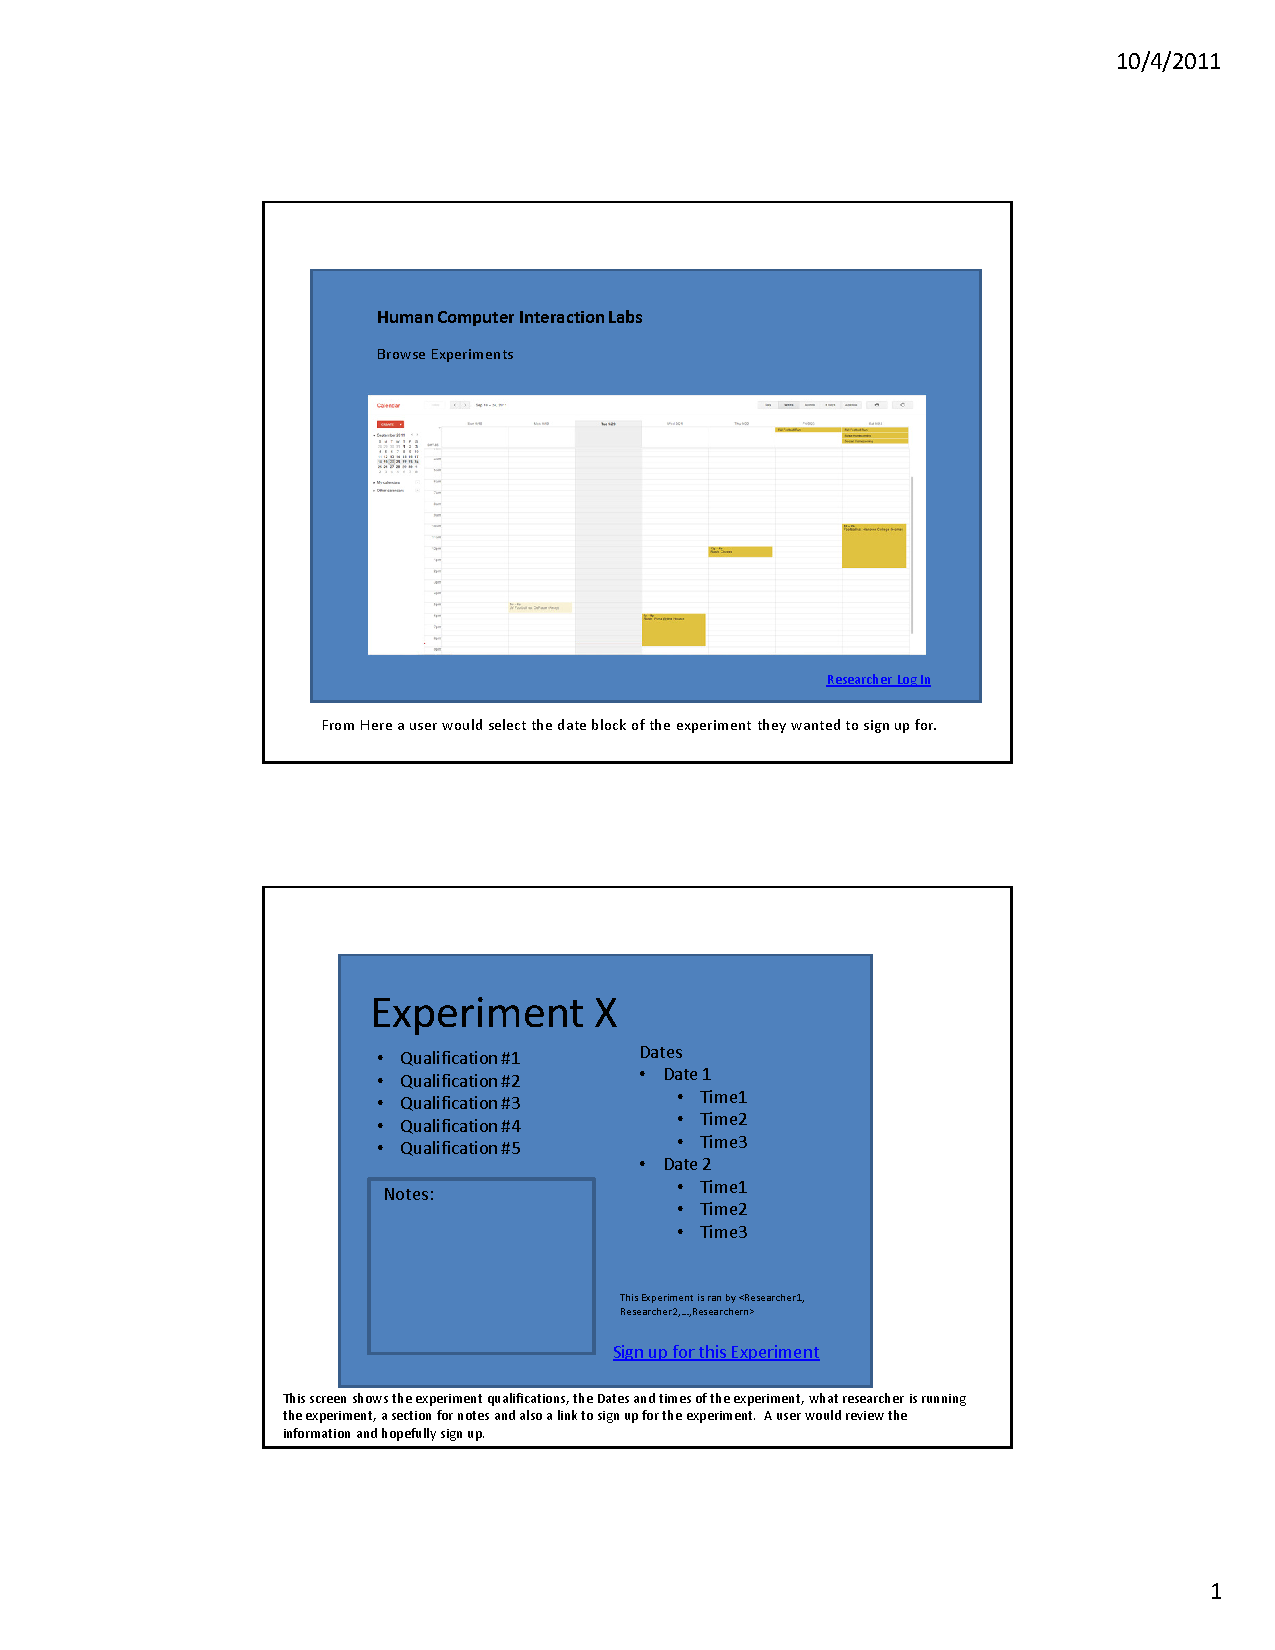
\includepdf[pages=-,pagecommand={}]{../other/allie/StoryBoardAllie2}
% fix for bibliography title
\renewcommand\refname{\section{References}}{\vspace*{-12mm}}
\bibliographystyle{plain}
\bibliography{bibliography}

\section{Appendix}

\section{Glossary}

\section{Index}

\end{document}